\subsection{Pujoskaavion synty: alkuperäinen}
Kuten edellisessä solmuja ja linkkejä käsittelevässä kappaleessa esiteltiin, linkkien yhteen pujominen ei operaationa manipuloi linkkejä, vaan itse asiassa ympäröivää avaruutta. Solmut, joiden kautta kaksi linkkiä pujotaan yhteen, poistetaan avaruuksistaan, ja jäljelle jää kaksi tyhjää silmukkaa. Lopuksi avaruudet liimataan intuitionvastaisella tavalla yhteen tyhjiä silmukoita pitkin. Monesti pujomisen visuaalinen hahmottaminen on äärimmäisen hankalaa. Tärkeää on huomata, että operaatiota pitää ajatella abstraktina \emph{pujomisena}, eikä missään nimessä konkreettisena \emph{pujottamisena}.

\begin{oivallus}
    Ensimmäinen ja kenties keskeisin pujoskaavioihin liittyvä oivallus onkin, että kaavion ei pitäisi esittää ainoastaan solmua, vaan myös sitä ympäröivää avaruutta: miten avaruutta on edellisissä pujoksissa venytetty ja runnottu.

    Tätä varten kaavioon tarvitaan kahdenlaisia kaaviokomponentteja: avaruutta kuvaavia ja linkin osasia kuvaavia. Kokemus osoittaa, että niitä tarvitaan kolme.
    \begin{figure}[h!]
        \centering
        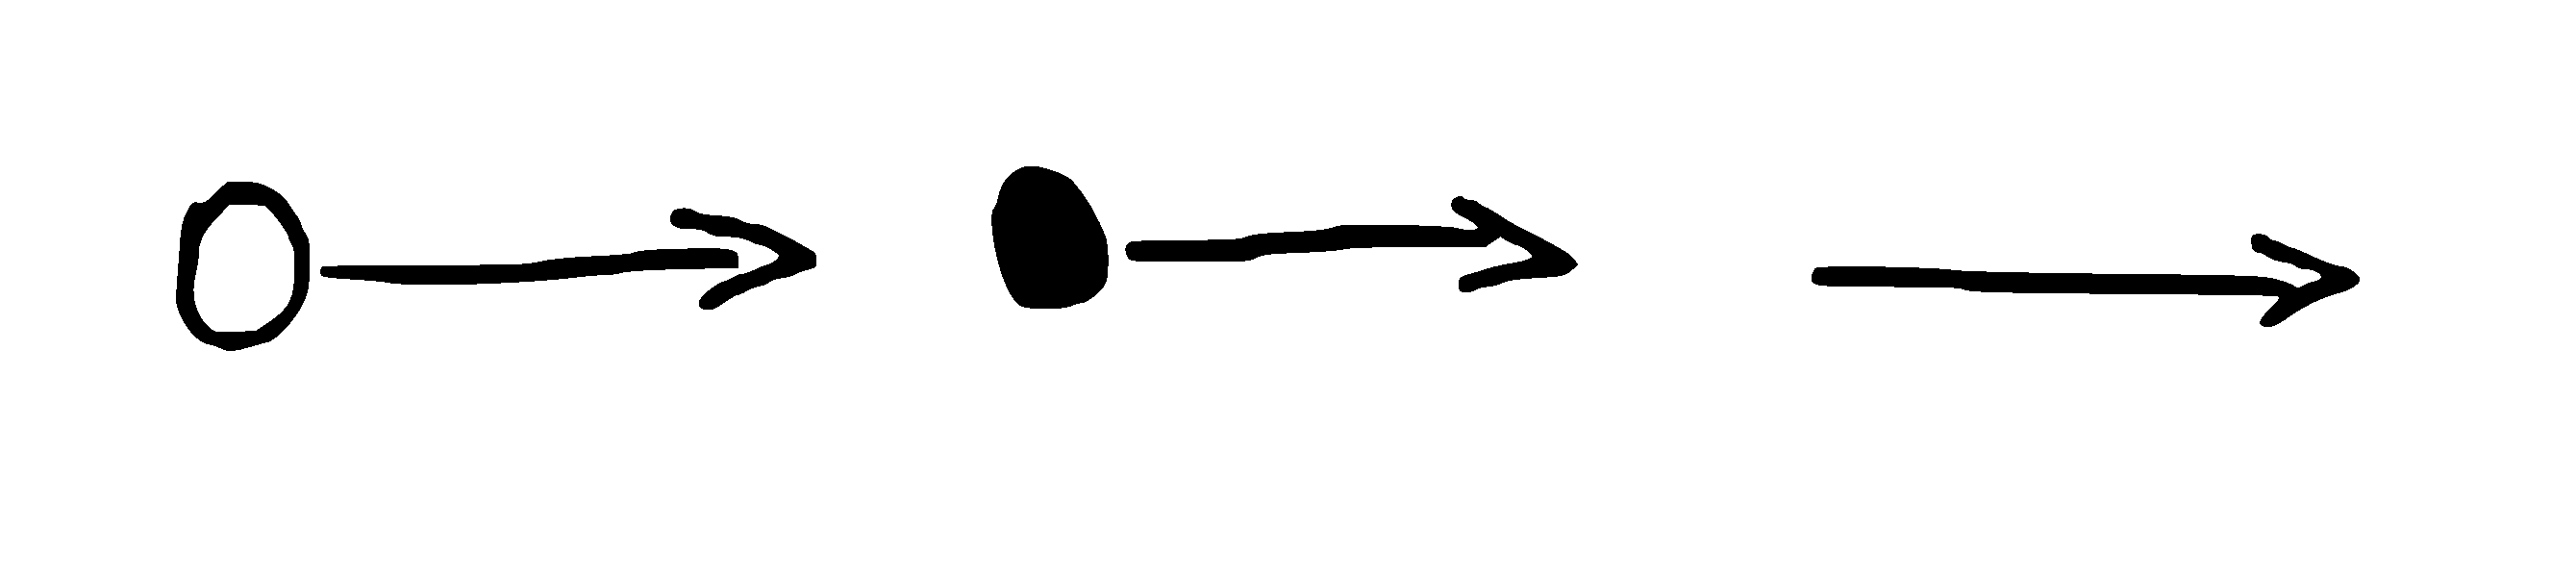
\includegraphics[width=0.5\textwidth]{figures/erityyppiset-nuolet.pdf}
        \label{kuva:erityyppiset-nuolet}
    \end{figure}
    Merkitään (vasemmalta oikealle) näitä tekstin seassa $\circ$, $\bullet$ ja $\rightarrow$.
\end{oivallus}

\begin{oivallus}
    Toinen oivallus ammentaa avaruuden rakenteesta. Käyrä, joka hajaantuisi $\R^3$:ssa positiiviseen ja negatiiviseen äärettömyyteen, ei voi käyttäytyä samoin $\pallo^3$:ssa, koska $\pallo^3$ on kompakti; käyrä tulee ennen pitkää takaisin lähtöpisteeseensä muodostaen $\pallo^3$:n globaalissa geometriassa ``silmukan''. Toisaalta ``silmukan'' voi muodostaa helpomminkin menemällä lokaalisti ympäri. Globaali ja lokaali silmukka ovat perustavalla tavalla erilaisia (vai ovatko? ts. samoin kuin lineaarisesti riippumattomat vektorit?); sanotaan että $\pallo^3$:lla on kaksi \emph{torusakselia}. 
    
    Kuvassa~\ref{kuva:torusakselit} on kaksi avaruutta. Ensimmäisessä on kaksi erilaista torusakselia. Jos toisen renkaan poistaa, jäljelle jäävää ei voi kutistaa pisteeksi. Jälkimmäisessä avaruudessa voi, joten torusakselit ovat samankaltaisia.
    \begin{figure}
        \centering
        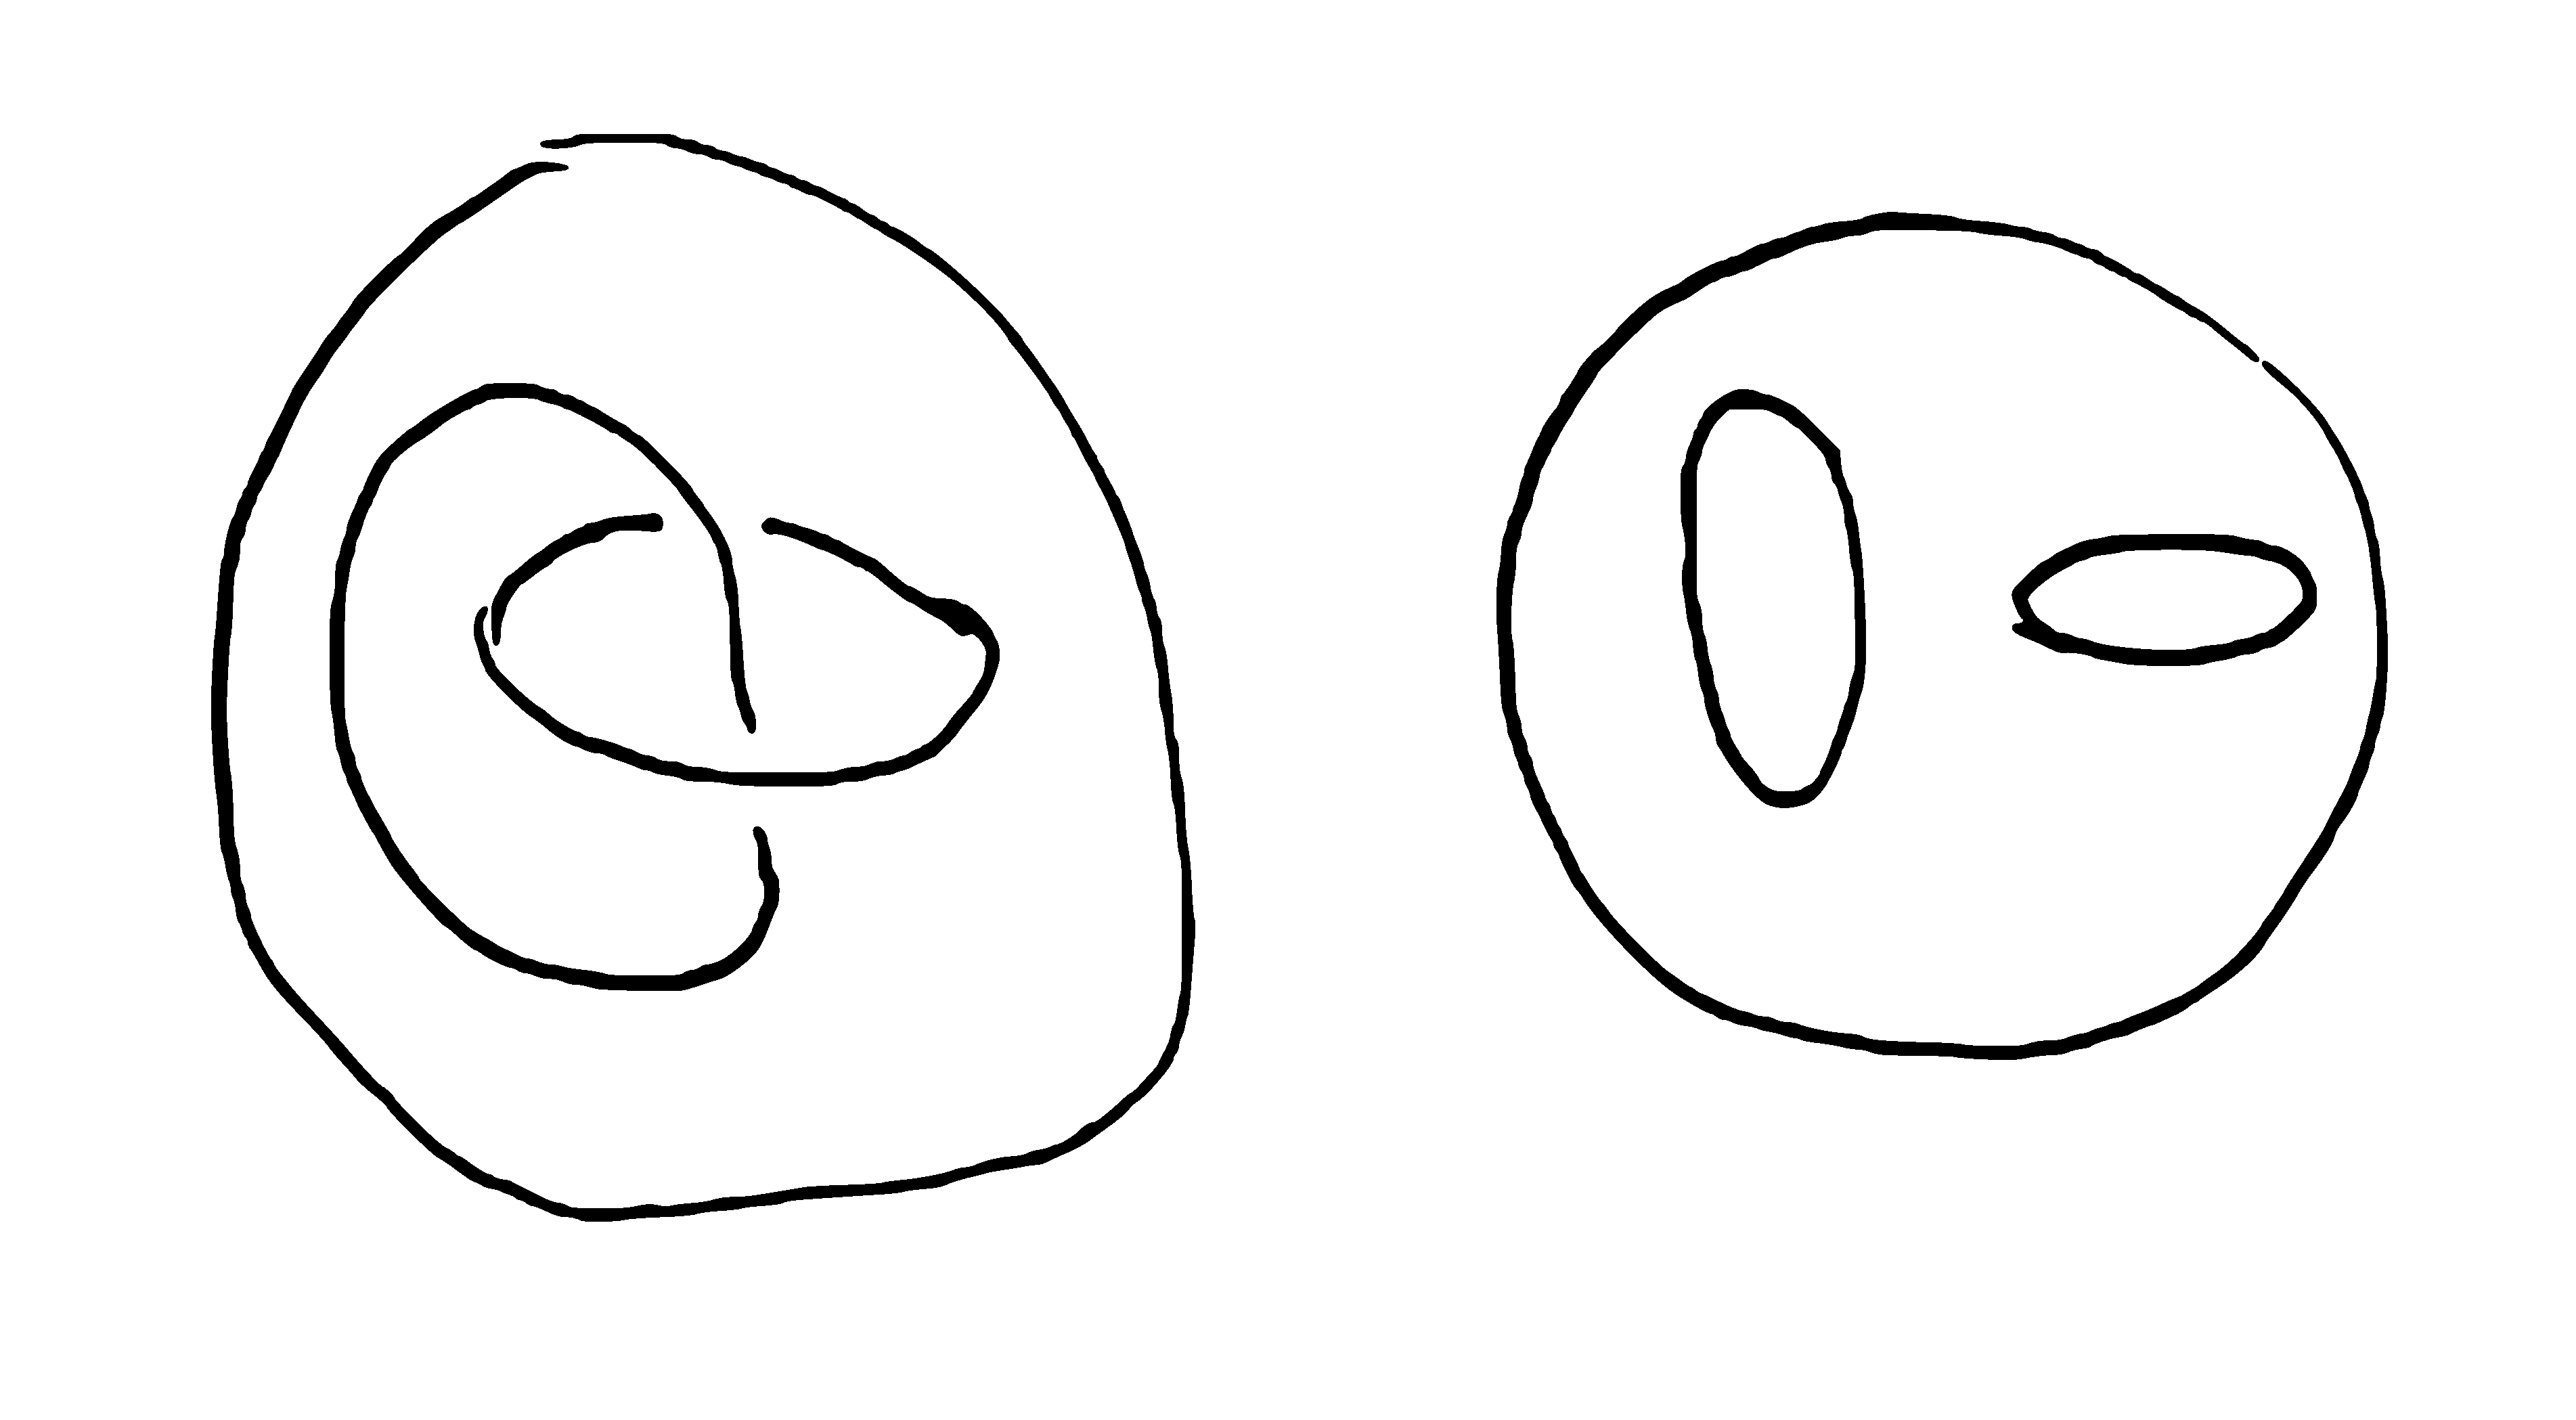
\includegraphics[width=0.5\textwidth]{figures/erityyppiset-ja-samantyyppiset-torusakselit.pdf}
        \caption{Kaksi erityyppistä ja samantyyppistä torusakselia.}
        \label{kuva:torusakselit}
    \end{figure}

    On olemassa myös avaruuksia, joilla on useampi torusakseli (vai olenko ymmärtänyt ``exceptional fibre'' -jutun ihan väärin?). Työn kannalta tärkein tällainen luokka ovat \emph{homologiset $n$-pallot}:
    \begin{quote}
        \textbf{Määritelmä~\ref{maar:homologinen-n-pallo}.} \emph{Homologinen $n$-pallo} on topologinen avaruus, jonka homologiaryhmät ovat samat kuin $\S^n$:llä. 

        \noindent
        \textbf{Ajatus.} Ympyrä $\S^1$ ja kahdeksikko eivät ole homologisia keskenään. Ensimmäisellä on yksi reikä, kun jälkimmäisellä taas kaksi. Homologisella $n$-pallolla on samantyyppisiä reikiä kuin $\S^n$:llä, ja samankaltainen globaali rakenne.
    \end{quote}
    \begin{huomautus}
        Toista oivallusta tukee se, että kahta solmua pujotessa syntyvä avaruus on homologinen $n$-pallo, mikäli alkuperäiset avaruudet olivat. Kaikki toivotut hyvät ominaisuudet säilyvät pujonnassa.
    \end{huomautus}
\end{oivallus}

\begin{oivallus}
    Kolmas oivallus on, että voidaan käyttää avaruuden sisäisiä torusakseli-rakenteita hyväksi torussolmujen esittämisessä. Esimerkiksi tyypin $(p,q)$ torussolmun voi ajatella käyränä, joka kiertää $\S^3$:n yhden torusakselin $p$ kertaa ja toisen torusakselin $q$ kertaa ennen palaamistaan lähtöpisteeseen.
\end{oivallus}

Kun nämä oivallukset kootaan yhteen, voidaan yksinkertaisin epätriviaali torussolmu $(2,3)$ esittää kuten kuvassa ??.